\setcounter{section}{4}

\Needspace{5\baselineskip}
\hypertarget{diffusion-forcing-and-roll-forcing}{%
\section{Diffusion Forcing and Roll Forcing}\label{diffusion-forcing-and-roll-forcing}}

\Needspace{5\baselineskip}
\hypertarget{i.-diffusion-forcing}{%
\subsection{I. Diffusion Forcing}\label{i.-diffusion-forcing}}

\Needspace{5\baselineskip}
\hypertarget{background}{%
\subsubsection{(1) Background}\label{background}}

Conventional sequence modeling has two main extremes.

\begin{itemize}
\tightlist
\item
  Next-token prediction models (teacher forcing): models such as GPT support variable-length generation, but error accumulation often causes prediction collapse on continuous data such as video. Because they commit to the future step by step, future rewards or goals cannot guide the current step.
\item
  Full-sequence diffusion models: commonly used for video generation or offline RL planning. They add the same noise level to all time steps as a whole. Although this supports multistep guidance, the noncausal architecture generates only fixed-length sequences and cannot make decisions based on causal uncertainty as humans do.
\end{itemize}

Most current models combining diffusion and autoregression generate in blocks: given generated blocks \(x_1,\ldots,x_t\), a diffusion model generates a new block \(x_{t+1}\) from noise. The implicit assumption is that every block has the same noise level. Diffusion Forcing instead assigns an independent, random noise level to every token or block and trains a causal model to unmask them.

\Needspace{5\baselineskip}
\hypertarget{training-phase}{%
\subsubsection{(2) Training phase}\label{training-phase}}

\Needspace{5\baselineskip}
Diffusion Forcing trains the model to denoise sequences with arbitrary, independent noise levels. The workflow is:

\begin{enumerate}
\def\labelenumi{\arabic{enumi}.}
\tightlist
\item
  Sample a real observation sequence \((x_1,\ldots,x_T)\) from the dataset.
\item
  Assign independent noise: for \(t=1,\ldots,T\), independently and uniformly sample a noise level \(k_t\in\{0,1,\ldots,K\}\) for each \(x_t\).
\item
  Forward noise addition: diffuse each token to its assigned noise level, obtaining observation \(x_t^{k_t}\) and computing target noise \(\epsilon_t\).
\item
\Needspace{5\baselineskip}
  Hidden-state update and noise prediction: predict noise from the previous hidden state \(z_{t-1}\), current noisy observation \(x_t^{k_t}\), and noise level \(k_t\):
\end{enumerate}

\[
\hat{\epsilon}_t=\epsilon_\theta(z_{t-1},x_t^{k_t},k_t)
\]

Also update the new state \(z_t\).

\begin{enumerate}
\def\labelenumi{\arabic{enumi}.}
\setcounter{enumi}{4}
\tightlist
\item
  Backpropagation: compute MSE between predicted and actual noise at all time steps and update network weights \(\theta\).
\end{enumerate}

\Needspace{5\baselineskip}
\hypertarget{inference-control-through-a-scheduling-matrix}{%
\subsubsection{(3) Inference: control through a scheduling matrix}\label{inference-control-through-a-scheduling-matrix}}

\Needspace{5\baselineskip}
In the algorithm, the scheduling matrix \(K\) is an \(M\times T\) two-dimensional grid:

\begin{itemize}
\tightlist
\item
  Columns (\(T\)): sequence time steps, \(t\in\{1,2,\ldots,T\}\).
\item
  Rows (\(M\)): denoising sampling iterations, indexed by \(m\).
\item
  Element \(K_{m,t}\): each \(K_{m,t}\in\{0,1,\ldots,K\}\) specifies the exact target noise level that token \(t\) must reach in denoising iteration \(m\). \(K\) means pure white noise; \(0\) means clean data.
\end{itemize}

\Needspace{5\baselineskip}
During inference, the model follows this matrix like a musical score. The procedure is:

\begin{enumerate}
\def\labelenumi{\arabic{enumi}.}
\tightlist
\item
  Global initialization: initialize the entire target sequence \(x_{1:T}\) as independent Gaussian white noise, with every token at noise level \(K\).
\item
  Outer loop (row-wise denoising): traverse the matrix rows, for example from \(M\) down to \(0\). Each row is one global denoising update.
\item
  Inner loop (causal progression): within row \(m\), traverse time \(t=1,\ldots,T\) from left to right.
\item
  Read the target and denoise one step: for \((m,t)\), read \(k=K_{m,t}\). Using current hidden state \(z_{t-1}\) and \(x_t\) with its actual current noise, predict \(\epsilon_\theta(z_{t-1},x_t,k)\), then use a Langevin dynamics formula or DDIM to reduce \(x_t\) precisely to target noise level \(k\).
\item
  Causal state update: update hidden state \(z_t\) from the newly denoised \(x_t\). Under the causal architecture, updated \(z_t\) contains the latest information about \(x_{1:t}\) and passes to time step \(t+1\).
\end{enumerate}

\Needspace{5\baselineskip}
\hypertarget{generation-paradigms-based-on-the-scheduling-matrix}{%
\subsubsection{(4) Generation paradigms based on the scheduling matrix}\label{generation-paradigms-based-on-the-scheduling-matrix}}

Scheduling matrix \(K\) supports three typical paradigms.

\hypertarget{full-sequence-diffusion-mode}{%
\paragraph{1. Full-sequence diffusion mode}\label{full-sequence-diffusion-mode}}

To imitate conventional video diffusion, such as part of the logic of SVD or Sora, make all entries in each row identical. Every token is uniformly denoised in synchrony, approximating conventional full-sequence diffusion.

\hypertarget{autoregressive-mode}{%
\paragraph{2. Autoregressive mode}\label{autoregressive-mode}}

To imitate word-by-word language generation, make the matrix move in a staircase pattern: begin generating the next token only after the preceding token and its noise floor reach 0. This preserves causal order and diffusion-style local refinement.

\hypertarget{causal-uncertainty-or-pyramid-scheduling}{%
\paragraph{3. Causal uncertainty or pyramid scheduling}\label{causal-uncertainty-or-pyramid-scheduling}}

This is the paper's core innovation. The matrix has a half-pyramid or zipper-like pattern: near-future noise is reduced more, while the distant future retains higher noise. The control principle is that, when \(x_1\) is predicted, \(x_2\) and \(x_3\) are not fully formed but carry traces of future planning trends. This matches Bayesian filtering's modeling of increasing future uncertainty in an uncertain world and allows information not yet manifested in the present to backpropagate smoothly to the current decision point, enabling planning guidance.

\textbf{Correspondence with Transformer architectures:}

In conventional autoregression, past tokens become fixed once generated, so future rewards cannot change past decisions. In Diffusion Forcing, future tokens remain highly noisy but can backpropagate gradients through the causal architecture's hidden state \(z_t\) to earlier tokens. The model can thus ``foresee'' distant-future rewards and correct its path in a present that has not yet been fully fixed.

\Needspace{5\baselineskip}
In Transformer attention, this can be understood through two mechanisms:

\begin{enumerate}
\def\labelenumi{\arabic{enumi}.}
\tightlist
\item
  Complete information occlusion (DF's distinctive fractional masking): changing the schedule can give future tokens partial noise, for example \(k=K/2\). A future token then becomes \(\sqrt{\bar{\alpha}_k}x^0+\sqrt{1-\bar{\alpha}_k}\epsilon\), containing both real future features \(x^0\) and noise. During self-attention, past tokens can extract attenuated future signals from the \(V\) matrix.
\item
  When a future token is pure noise, its key and value are almost random noise. Even if attention reads it, it obtains no real information, making this equivalent to a conventional causal mask.
\end{enumerate}

By controlling the future-token noise ratio, a Transformer can transition smoothly from fully noncausal to partly causal and then strictly causal without changing its network structure or designing complex attention masks.

The elegance of Diffusion Forcing is that noise is no longer merely an obstacle to remove: it becomes the core control medium for adjusting receptive fields, controlling causality and propagating planning gradients.

\Needspace{5\baselineskip}
\hypertarget{planning-with-monte-carlo-guidance}{%
\subsubsection{(5) Planning with Monte Carlo guidance}\label{planning-with-monte-carlo-guidance}}

In conventional full-sequence diffusion, all tokens have the same noise level, tying present and future to the same denoising trajectory. Sampling multiple futures while fixing the present is difficult. Diffusion Forcing allows future positions to remain noisier, so nearby current states can be fixed while future noise is resampled to produce multiple possible trajectories.

\Needspace{5\baselineskip}
Monte Carlo guidance (MCG) samples futures at every denoising step:

\begin{enumerate}
\def\labelenumi{\arabic{enumi}.}
\tightlist
\item
  Current observation: at the environment's current real time step, the agent has the historically accumulated hidden state \(z_{t-1}\).
\item
  Generate a look-ahead window: instead of planning indefinitely, set a future horizon \(H\). The model begins generating a local future sequence \(x_{t:t+H}\) in latent space.
\item
  MCG sampling at each denoising step: during every denoising iteration of local sequence \(x_{t:t+H}\), to decide how to denoise the current \(x_t^k\), branch into multiple uncertain future trajectories in latent space from \(t+1\) to \(t+H\).
\end{enumerate}

\Needspace{5\baselineskip}
Compute the expected future reward \(R^{(i)}\) of each of these \(N\) trajectories and average them:

\[
\bar{R}(x_t^k)=\frac{1}{N}\sum_{i=1}^N R^{(i)}
\]

\Needspace{5\baselineskip}
Then differentiate with respect to the current blurry input \(x_t^k\) being denoised:

\[
\nabla_{x_t^k}\bar{R}(x_t^k)
\]

This gradient means that moving the current noisy, blurry \(x_t^k\) slightly in its direction maximizes the probability of evolving into a high-reward future trajectory.

\Needspace{5\baselineskip}
Inject the future-reward gradient directly into noise prediction, similarly to classifier guidance:

\[
\begin{aligned}
\tilde{\epsilon}
&=
\epsilon_\theta(x_t^k,k_t)
\\
&\quad -
\eta\sqrt{1-\bar{\alpha}_{k_t}}\nabla_{x_t^k}\bar{R}(x_t^k)
\end{aligned}
\]

Use the corrected noise \(\tilde{\epsilon}\) to denoise \(x_t^k\) to the next clearer level \(x_t^{k-1}\).

In MCG, the \(N\) sampled future trajectories are discarded after gradient computation. They serve only as temporary scouts, providing a lower-variance, unbiased estimate of the expected reward gradient.

After repeated denoising, current token \(x_t\), the action \(\hat{u}_t\) to execute now, becomes clear. The agent executes only this action in reality, then uses the environment's real reward \(r_t\) and next observation \(o_{t+1}\) for the next round of rolling planning. This is consistent with model predictive control (MPC).

In this way, throughout the long process of reducing the current action from pure noise to 0, every step is pulled by expected future gradients. When noise reaches 0, the action already lies on a route to the optimum. This method is highly sample-efficient and produces smoother, more physically consistent trajectories.

\Needspace{5\baselineskip}
\hypertarget{why-can-this-architecture-send-future-gradients-into-the-past-when-conventional-autoregression-and-diffusion-cannot}{%
\subsubsection{(6) Why can this architecture send future gradients into the past when conventional autoregression and diffusion cannot?}\label{why-can-this-architecture-send-future-gradients-into-the-past-when-conventional-autoregression-and-diffusion-cannot}}

Autoregression's bottleneck is committing too early. It must fully determine the current token, for example through distribution sampling, argmax or temperature sampling, before feeding it in as historical context to predict future \(x_{t+1}\). Once this hard commitment is made, the current state is finished, so future rewards cannot update it through gradients.

Pure diffusion's bottleneck is an inability to branch. In full-sequence diffusion, fixing the current noisy state \(x_t^k\) while all positions continue denoising at the same level fixes the whole computation graph. Only one deterministic future trajectory tightly tied to the present is obtained. With very high trajectory variance, this gradient can also be unstable.

\Needspace{5\baselineskip}
Diffusion Forcing preserves both future uncertainty and present differentiability:

\begin{enumerate}
\def\labelenumi{\arabic{enumi}.}
\tightlist
\item
  Future noise is much higher than current noise. The future is therefore not locked in: we can freeze the current \(x_t^k\) and inject hundreds or thousands of different white-noise samples into the future to produce enough branches.
\item
  The current token has not been hard-committed as in autoregression and remains slightly noisy, for example at \(k=2\). As a continuous, uncertain variable, it can receive the expected-reward gradient directly, smoothly changing its denoising direction in subsequent Langevin dynamics.
\end{enumerate}

\Needspace{5\baselineskip}
\hypertarget{slightly-noising-historical-information}{%
\subsubsection{(7) Slightly noising historical information}\label{slightly-noising-historical-information}}

For extremely long sequences, Diffusion Forcing exploits sampling flexibility with a clever error-accumulation safeguard: slightly noising history.

When generating frame \(x_t\), DF does not fully trust the previous frame \(x_{t-1}\) because it is self-generated and necessarily contains small imperfections. Instead, it retains a previous-frame hidden state \(z_{t-1}\) with very small noise \(k_{\mathrm{small}}\), for example \(K_{\mathrm{small}}\ll K\), and conditions the next frame on it. Because the model learned from noisy inputs during training, this keeps autoregressive generation in distribution, enabling stable rollouts of unlimited length and completely resolving collapse in conventional teacher-forcing models.

\Needspace{5\baselineskip}
\hypertarget{proof-of-theoretical-feasibility}{%
\subsubsection{(8) Proof of theoretical feasibility}\label{proof-of-theoretical-feasibility}}

Appendix A provides a rigorous ELBO-based mathematical proof. The model optimizes a modified weighted ELBO. Assume the forward Markov process is \(q(x^{1:K}|x^0)=\prod_{k=1}^K q(x^k|x^{k-1})\) and the generative model is parameterized by \(p_\theta\). The authors prove that DF training maximizes a lower bound on the true joint log-likelihood.

\Needspace{5\baselineskip}
By Theorem A.1, for independently sampled noise levels \(k_{1:T}\), the ELBO of the expected log-likelihood is:

\[
\begin{aligned}
&\mathbb{E}_{\mathrm{forward}}
\left[
\log p_\theta\left((x_t^k)_{1\le t\le T}\right)
\right] \\
&\quad \ge \mathcal{C}(x_{1:T}^0)
+\mathbb{E}_{\mathrm{forward},p_\theta,z_{1:T}}
\left[
\sum_{t=1}^T
\right. \\
&\qquad \left.
\left(
\frac{1}{K+1}\log p_\theta(x_t^0\mid z_{1:t},z_{t-1})
+\sum_{j=2}^K\frac{j}{K+1}
\right.
\right. \\
&\qquad\qquad \left.\left.
{}\cdot D_{\mathrm{KL}}\left(
q(x_t^{j-1}\mid x_t^j,x_t^0)
\middle\|
p_\theta(x_t^{j-1}\mid x_t^j,z_{t-1})
\right)
\right)
\right]
\end{aligned}
\]

The key finding is that, when latent state \(z_{t-1}\) has sufficient expressive power, the loss terms across time steps \(t\) decouple, so weights \(\frac{j}{K+1}\) can be omitted or reweighted. The final objective becomes the familiar diffusion least-squares form:

\[
\mathcal{L}(\theta)=
\mathbb{E}_{k_{1:T},x,\epsilon}
\left[
\sum_{t=1}^T
\left\|
\epsilon_t-\epsilon_\theta(z_{t-1},x_t^{k_t},k_t)
\right\|^2
\right]
\]

Because the loss covers all possible local masking patterns in the sequence, the model can sample subsequence marginal distributions of real data using any time-step schedule at inference.

\Needspace{5\baselineskip}
\hypertarget{ii.-rolling-forcing-rolling-denoising-generation}{%
\subsection{II. Rolling Forcing: Rolling Denoising Generation}\label{ii.-rolling-forcing-rolling-denoising-generation}}

For streaming long-video generation, Self Forcing resolves the train--test mismatch but not error accumulation completely. Rolling Forcing aims to address this.

\begin{enumerate}
\def\labelenumi{\arabic{enumi}.}
\tightlist
\item
  \textbf{Joint denoising in a sliding window}: instead of denoising frame by frame, denoise jointly within a sliding window. The \(T\) frames in the window receive increasing noise levels, from almost clear to pure noise. Bidirectional attention lets relatively clear frames guide highly noisy ones, suppressing errors locally before they propagate to the next frame. Each forward pass outputs only the clearest frame, then shifts the whole window forward.
\end{enumerate}

\begin{figure}[htbp]
\centering
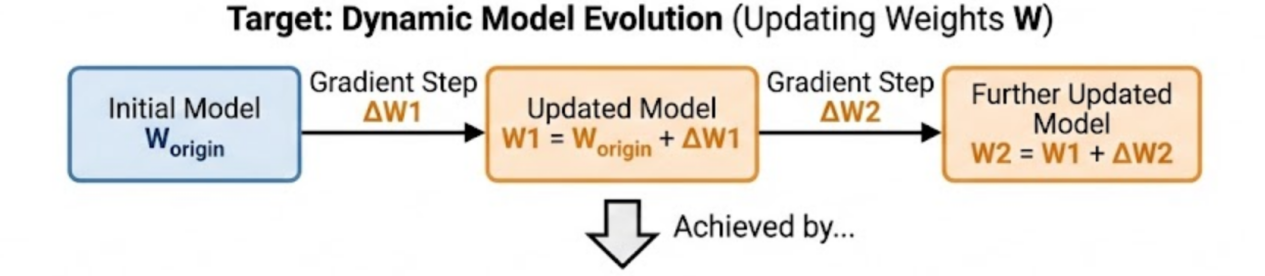
\includegraphics{images/image-0044.png}
\caption{Comparison of sequence generation in Diffusion Forcing and Rolling Forcing}
\end{figure}

\begin{figure}[htbp]
\centering
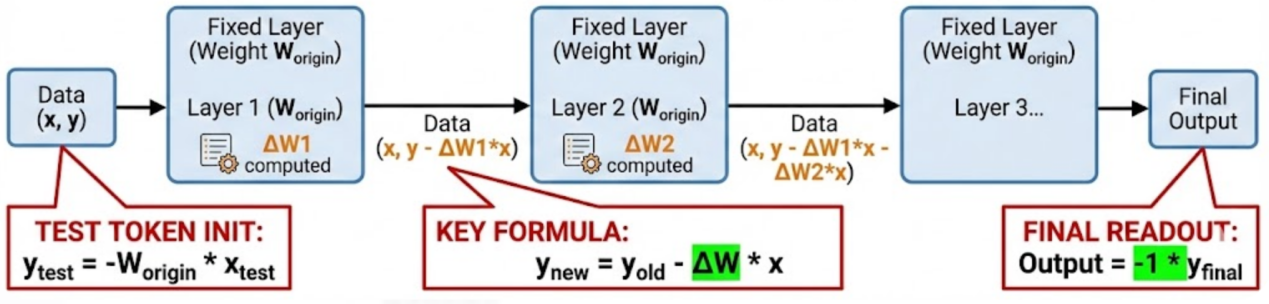
\includegraphics{images/image-0045.png}
\caption{Meaning of the colors and attention connections in the diagram}
\end{figure}

\begin{enumerate}
\def\labelenumi{\arabic{enumi}.}
\setcounter{enumi}{1}
\item
  \textbf{Attention sink}: cache the key-value states of the first few video frames as ``global context anchors,'' ensuring that, however far generation proceeds, the model can look back at the initial state. This strongly preserves global style, color tone and related information.
\item
  \textbf{Hybrid training}: combine RF's rolling-window objective with SF's frame-by-frame objective. SF acts as a regularizer here, preventing unnatural camera motion caused by the rolling-window mechanism.
\end{enumerate}

\FloatBarrier
\Needspace{5\baselineskip}
\hypertarget{references-142}{%
\subsection{References}\label{references-142}}

\vspace{0.25em}
\begin{itemize}
\tightlist
\item
  Chen, B., Monso, D. M., Du, Y., Simchowitz, M., Tedrake, R., \& Sitzmann, V. (2024). \href{https://arxiv.org/abs/2407.01392}{Diffusion Forcing: Next-token Prediction Meets Full-Sequence Diffusion}. NeurIPS.
\item
  Liu, K., Hu, W., Xu, J., Shan, Y., \& Lu, S. (2025). \href{https://arxiv.org/abs/2509.25161}{Rolling Forcing: Autoregressive Long Video Diffusion in Real Time}. ICLR.
\end{itemize}

\clearpage
